\section{Pulsed Laser Deposition}
The investigation of thin films is essential in science and 
technology and has led to countless inventions such as integrated circuits, 
microchips and many more. 
Therefore, it is crucial to have a reliable and precise way to fabricate thin films. 
One method, which is not only reliable, but also flexible and comparatively inexpensive,
is \ac{pld}. 
Therefore, this protocol aims to present the \ac{pld} structure and its working
principles.

\subsection{The PLD Process explained in steps}
In \ac{pld}, the process begins with a bulk material that will form the thin film.
This material source, called target, is installed into a vacuum chamber along with a 
substrate that serves as the foundation and growth template of the film.
For this lab course, a \ce{ZnO} target and a c-sapphire substrate was used.
A high-power pulsed laser in the ultraviolet spectral range is focused through a lens 
and directed through a window into the vacuum chamber, where it hits the target. 
During every laser pulse, the target material begins to ablate and vaporizes. 
The vaporized material interacts with the laser photons as well and thus excites into a 
plasma. 
This plasma is directed towards the substrate, where it condenses.
After each pulse, some material is added and after a fixed number of pulses,
a thin film is deposited on the substrate. 

The laser-target interaction is a complex and nonequilibrium process and therefore
hard to model analytically.
Laser photons are absorbed by the target material and excite the electronic system.
Due to the electron phonon interaction, this electronic excitation is converted 
into thermal, chemical and mechanical energy and leads to the ablation and evaporation
of the material.
The ejected species expand into the vacuum, interact with the laser and form a plasma
plume. 
This plume consists of electrons, atoms, ions, molecules and clusters and is directed 
towards the substrate.

\Ac{pld} runs inside a vacuum chamber under ultrahigh vacuum or under a controlled 
background gas pressure.
The background gas can be chosen, oxygen, nitrogen or argon are common candidates.
The substrate is normally heated using a resistive or laser heater.

\Ac{pld} is very flexible for investigating thin film materials.
It is applicable for a large material library, including oxides, nitrides and even
metals. 
For most materials it also ensures stoichiometric transfer from the target to the film,
but this is not guaranteed.

\subsection{Design of a \ac{pld} System}
In this section the structure of a \ac{pld} system shall be discussed.
\ac{pld} is a \ac{pvd} technique and thus characterized by a process in which the target
material transitions from a condensed phase to a vapor phase and then back to a thin 
film condensed phase on a substrate.
The vaporization process in accomplished by pulsed laser rays hitting the target inside
a vacuum chamber. 
Therefore, the laser and the chamber are  two main components that will be
explained in detail.

\subsubsection{Laser}
The most useful wavelengths for laser-induced ablation are in the range between
\qtyrange{200}{400}{\nano \meter}. 
In this region, most materials have a strong absorption and therefore a reduced 
penetration depth into the target. 
With that, thinner layers can be ablated, which generally increases thin film quality.
One should install an adjustable lens into the beam path to focus the laser beam onto 
the target with a known spot size.

Additionally, Commercially lasers in this spectral range are available and matured.
The two mail lasers are Nd:YAG and excimer lasers.
\paragraph{Nd:YAG Lasers}
are solid-state systems, with an yttrium aluminum garnet host (\ce{Y3AlO12})
crystal.
This crystal is doped with neodymium ion ($\ce{Nd^{{3+}}}$) impurities, that serve as an
active medium.
The neodymium ions inside the YAG crystal are excited by flashlamps and can 
relax into energetically lower states by photonic emission. 
The YAG crystal itself is not participating in photon emission.
This process leads to an emission of \qty{1064}{\nano\meter} photos.
With nonlinear crystal, this can be transformed to \qty{266}{\nano\meter} radiation.
The interaction with nonlinear crystal resuslts in a significant attenuation of intensity,
with only \qty{20}{\percent} of the original intensity remaining after transmission 
through the crystal.

\paragraph{Excimer Lasers} are gas lasers that emit photons directly in the ultraviolet 
spectral range.
A molecular gain medium is used, that has a metastable upper electronic state (excimer) 
and a repulsive ground state.
Through electric discharge, the constituents create excited species and can react to
excimer molecules.
These molecules can relax by induced emission and emit photons.
Due to the repulsive ground state, the ground state molecule is not stable and
dissociates into its components.

The most common excimer laser are krypton fluoride (\ce{KrF}) lasers.
A gas mixture of krypton and fluorine is pumped into the gas chamber. 
The formation of excimer molecules are complex and consists of several steps.
The most important reactions are listed below:
\begin{align*}
	\ce{Kr + e- &-> Kr+, Kr^*, Kr_2^+} \\
	\ce{F2 + e- &-> F + F-} \\
	\ce{Kr+ + F- + X &-> KrF^* + X} \\
	\ce{Kr_2^+ + F- &-> KrF^* + Kr} \\
	\ce{Kr^* + F2 &-> KrF^* + Kr} \\
	\ce{KrF^* &-> KrF + h\nu}
\end{align*}
In the preceded equations, $X$ is a third body that is needed for the reaction to occur,
and stabilize the excimer. 
This can be another noble gas like argon or neon.

\subsubsection{Vacuum Chamber}
\begin{figure}[h!]
	\centering
	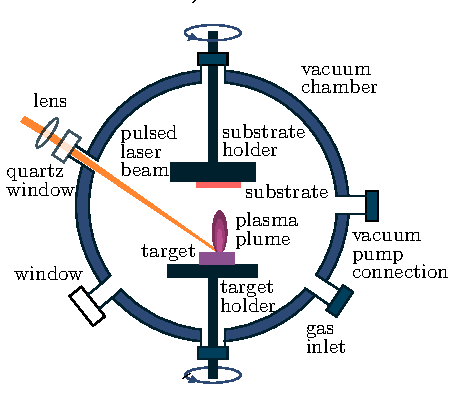
\includegraphics{../assets/pld_chamber}
	\caption{Schematic design of a \ac{pld} chamber.}
	\label{fig:pld_chamber}
\end{figure}
A possible configuration of a \ac{pld} vacuum chamber is shown in 
\cref{fig:pld_chamber}.
The chamber is equipped with a quartz window, used as a laser beam entrance.
Other viewport windows are beneficial for maintenance and monitoring and should
be installed.
These windows should be kept clean to ensure a high transmission of the laser beam
as well as a clear view into the chamber.

There is a vacuum pump connection and gas inlets to regulate a defined
vacuum or atmosphere.
Inside the chamber there are target and substrate holder, that can be rotated and
translated. 
The substrate holder offers various substrate clamps for different substrate sizes.
Usually, a resistive or laser heating system is installed near the substrate holder to
manipulate the substrates temperature and thus the quality of the deposited thin film.
To achieve a more even temperature distribution, the substrate holder is able to rotate.

Towards the substrate holder, a target holder is installed.
This holder is able to rotate and translate as well.
Advanced systems have a target carousel, that can hold multiple targets and can be
rotated to select the desired one.

\subsection{Detailed Working Principle Analysis}
After the \ac{pld} system design has been discussed, the working principle of the
\ac{pld} process shall be explained in detail.
The process can be divided into three main steps: the formation of the laser plasma,
the composition and expansion of the plasma and the nucleation and growth of the film.

\subsubsection{Ablation Process}
Using an adjustable lens, the laser beam is focused onto the target 
with a power density of \qty{10e8}{\watt\per\centi\meter\squared}.
This density is far above the materials thermal evaporation threshold, which is usually 
in order of \qty{10e7}{\watt\per\centi\meter\squared}.
As a result, the target material is ablated and vaporized.
This ablation process is complex and nonequilibrium due to the discontinuous nature 
of the laser pulses.

Thermal ablation by absorption of the laser photons is the most common ablation 
mechanism:
The laser photons are absorbed by the target material.
Due to the high energy of the laser photons, the target material ionizes and 
free electrons are generated.
These free electrons oscillate and can collide with the atoms of the bulk material,
thus transferring energy to the lattice of the target material.
Electromagnetic energy is converted into thermal and chemical energy.
The material is heated up and begins to vaporize.

Apart from thermal ablation, nonthermal, photoinduced electronic sputtering can occur.
This mechanism is based on the direct interaction of the laser photons with the 
electronic system.
Due to electron excitation, chemical bonds can be broken and the material is ejected
from the target, without any significant change in temperature.

Droplets and flakes can be expelled from the target towards the substrate as a result
of plasma recoil pressure and thermal shocks. 
This leads to a reduction of thin film quality.

The target surface is altered during the ablation process, which results in target 
erosion.
This leads to a deviation of the surface normal, therefore changing the plasma 
plume direction.
In order to ensure a uniform material removal, the target is rotated and translated.

\subsubsection{Plasma formation and expansion}
After the material is vaporized, it starts interacting with the laser photons too.
As a result, the material is excited and ionized and a plasma plume is formed.
Due to Coulomb interaction and recoil from the target surface, 
the plasma expands perpendicular to the target surface.

The spatial dependence of the plume depends strongly on the background gas pressure.
At a low background pressures around \qty{10e-4}{\milli \bar} or lower, the plume is
narrow and its constituents have a high velocity.
Only a few scattering events occur.

At intermediate pressures, between \qtyrange{10e-3}{10e-2}{\milli \bar}
a splitting of high energetic ions from less energetic species can be observed.
In high-pressure regions with a background pressure of \qty{10e-1}{\milli \bar} or 
higher, the expansion of the plasma is diffusion-like.
At higher pressures, the plasma plume is wider and the velocity of the species is
reduced.
To underline the influence of the background pressure, the maximum kinetic 
energy of ions with a background pressure of \qty{10e-2}{\milli \bar} is around
\qty{30}{\kilo \electronvolt}, while at \qty{10e-1}{\milli \bar} it is only
\qty{4}{\kilo \electronvolt}.
\begin{figure}
	\centering
	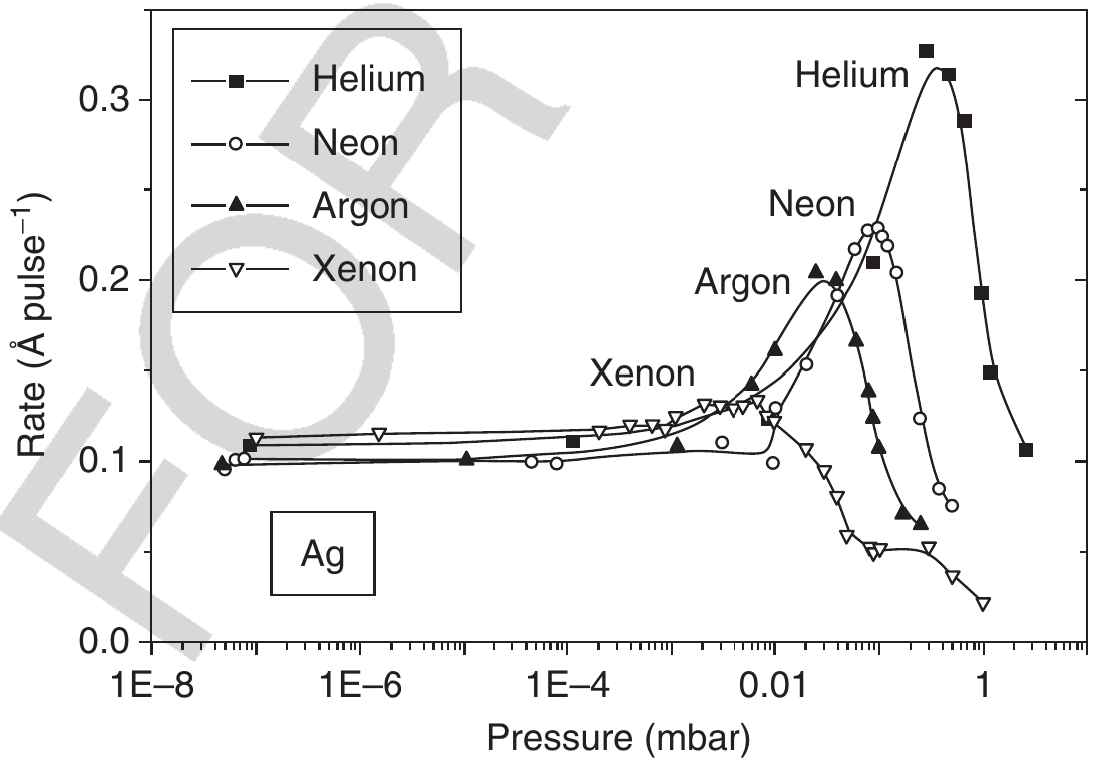
\includegraphics[width=0.98\columnwidth]{../assets/deposition_rate.png}
	\caption{Deposition rate as a function of background pressure for helium, neon, 
	argon and xenon background gases.}
	\label{fig:pld_plasma}
\end{figure}
Not only the kinetic energy of the species is influenced by the background pressure,
but also the deposition rate. 
In \cref{fig:pld_plasma} the deposition rate is shown as a function of the background
pressure for different background gases.
It can be seen that the deposition rate for low background pressures is low.
This is due to the high constituents velocity, which leads to resputtering of the
deposited material.
At higher background pressures, the particle velocity is reduced and the deposition
rate increases.
For even higher pressures, the deposition rate decreases again, 
as a result of the slower and wider spread plasma plume.
Background gas pressure can also lead to a change in stoichiometry of the deposited 
film.
Especially the oxygen concentration in oxide films is strongly influenced by the
background pressure.

\subsubsection{Nucleation and Growth of the Film}
### Deposition of Ablated Material, Nucleation, and Growth of the Film
- condensation of plasma at substrate surface
- nucleation into solid structure
- film growth
- essential for structural quality
- high-energetic species bombarding the substrate
- causing defekt formation
- forming near-surface collision region which serves as source for condensation
- film nucleates and grows on substrate surface
- laser parameter influencing nucleation process
	- ionization degree of ablated material is related to laser fluescence
	- affect film quality, stoichiometry and deposition flux
- substrate temeperature
	- nucleation density decreases as temperature is increased
- substrate surface
	- nucleation and growth can affect the surface preparation
- background pressure
	- oxygen for stochiometric transfer 
	- if oxygen background is too low, the film composition deviates from target composition including a considerable oxygen deficiency
- a large supersaturation occurs on the substrate during pulse
- material pulse causes large nucleation density on substrate surface
- the large density of adatoms induces a large density of nucleation centers
- Three growth modes
	- Layer-by-layer (Frank-van der Merwe)
		- islands with monoatomic nucleate until critical density is reached
		- with more material islands continue to grow laterally
		- run into each other (coalescence)
		- atoms diffuse into pits to complete the first monolayer
	- 5-30 laser pulses required to grow a monolayer
	- very precise control using in situ RHEED 
- 3D growth
	- once islands are formed, additional island nucleate on top, i.e. vertically
	- not layer by layer but three-dimensional islands
- step-flow 
	- single-crystalline substrates with miscut
	- miscut leads to atomic steps on surface
	- atoms land on surface and diffuse to a step edge
	- steps travelling across surface


\subsection{PLD in Comparison to other Thin Film Deposition Techniques}
\subsubsection{Sputtering}
\subsubsection{Thermal Evaporation}
\subsubsection{MBE}

\subsubsection{Drawbacks and Advantages compared to other Techniques}


- considerable material all within the chamber. especially in windows
	- leads to permanent damage


### Introduction
- basic equipment discussion
- PLD is versatile technique for wide range of thin films and multilayer structures
- attractive start-up cost
- thin film quality is comparable to molecular beam epitaxy 
- plasma energy source (laser) is independent from the deposition system
- reliable and userfriendly excimer lasers are already made
## Limitations of PLD and How to Overcome Them
### Trace Element Contamination
- trace element contamination of thin films is important issue
- quantum hall mobility of PLD heterostructure reaches far smaller maximum than high-purity MBE techniques
- PLD suffers from target preparation
	- ball mills
	- press molds
	- sintering ovens
	- source powders with low purities
- PLD suffers from construction alloy constituents
	- there are visible at edge positions (close to substrate holder)
### Droplets and Outgrows
- Particulates and globules, aka droplets, can be found in deposited film
- droplets have size of typically $\pu{ 1\mu m }$ range
- to avoid that
	- velocity filter
	- perpendicular target and substrate arrangement (only light plasma constituents are scattered towards substrate)
	- PLD setups with colloding plasma plumes
- droplet reduction often reduce deposition rate and make process more complicated

## Advantages of PLD
### Flexibility
- stoichiometric transfer of multielement compounds from a single target to substrat
- chemical composition of complex materials 
- oxygen content of oxide films can be easily controlled by background pressure
	- oxygen background gas can differ a lot
- most targets can be fabricated by simple lab equipment and available powders
- low daily running costs 
- laser as external energy source  and deposition chamber are separated
- clean process
- laser energy can be controlled independently from background pressure
- wide parameter space
## Industrial Upscaling
- high mass deposition on large areas
	- up to 8-inch diameter
- high laser pulse energy with high repetition rate
	- excimer laser performance high pulse energy and higher focus area with lower wavelength